% =====================================
% Purpose: Create a Robert Bringhurst style thesis paper using the 
% classicthesis package and some custom enhancements - this is 
% the default template for most of my documents
% =====================================

% =====================================
% Document Class and main packages
% =====================================

\documentclass[10pt,a4paper, hidelinks]{article} % KOMA-Script article scrartcl
\usepackage[nochapters, pdfspacing]{classicthesis} % [nochapters] [drafting] (puts date/time at bottom) [beramono] (changed mono spaced font)

% =====================================
% Packages in Use
% =====================================

%Math Packages
\usepackage{amsmath}
\usepackage{amsfonts}
\usepackage{amssymb}
\usepackage{nicefrac} % For typsetting inline fractions
\usepackage{mathtools} % For substack and mathclap (underbrace helper commands)
\usepackage{algpseudocode}
\usepackage{tcolorbox}
%\usepackage[]{algorithm2e}

%% Typography enhancements
\usepackage{microtype} % For awesome typographical improvements
\usepackage{booktabs} % Pretty \begin{tabular}
\usepackage{multicol} % For pretty multi-columns enviroments
\usepackage{xspace} % For use in a command to ensure proper spacing
\usepackage[margin=1in]{geometry}
%\usepackage{geometry} %uncomment this is you want full page documentation
\usepackage{graphicx} % for allowing pictures
\usepackage{float} % For the purpose of adding \begin{figure} [H]
\usepackage{lipsum} % For adding filler text
\usepackage{wasysym} % For the \newmoon command for the legal blobs
\usepackage{caption}
\usepackage{subcaption}
\usepackage{longtable}
% For commenting on incomplete or new items
\usepackage{todonotes} % \missingfigure{} is the best command
\usepackage{wrapfig}

% For inclusion of PDFs in the document \includepdf[pages={3,{},8-11,15}]{example.pdf}
% This will include page 3, a blank page, 8,9,10,11, and 15
% you can set this to draft to get boxes or final to get the default which includes
% the pages
% Options:
% 	fitpaper: Use this to insert the page as is - otherwise items are scaled to page
% 	rotateoversize: Attempt to rotate oversized pages and scale them
\usepackage[final]{pdfpages}

% =====================================
% Graphics 
% =====================================

% For quick graphics insert -- Full Line --
\newcommand{\qpic}[2]{
\begin{figure}[H]
\centering
\includegraphics[width=1\linewidth]{./#1}
\caption{#2}
\label{fig:#1}
\end{figure}
}

% For quick graphics insert -- Normal Size --
\newcommand{\qpics}[2]{
\begin{figure}[H]
\centering
\includegraphics[width=0.7\linewidth]{./#1}
\caption{#2}
\label{fig:#1}
\end{figure}
}

% =====================================
% Custom Macros that make life easier
% =====================================

% Description Enviroment Item Helper Commands
\newcommand{\im}[1]{\item[#1] \xspace}
\newcommand{\imp}[1]{\item[(#1)] \xspace}

% Auto-commas for long nominal and dollar amounts
\RequirePackage{siunitx}
\newcommand{\commasep}[1]{\num[group-separator={,}]{#1}}
\newcommand{\money}[1]{\$\commasep{#1}}
\usepackage{forest}
% Borrowing from tufte, this is the \newthought command that is 
% often used to bring about the change from one subsubsection
% to another and is a good way to bring things up logically into smaller
% bites
\newcommand{\newthought}[1]{
\vspace{11pt} \noindent
\spacedlowsmallcaps{#1}
}

% Code for the fast creation of bullet lists
\newcommand{\qb}[1]{\begin{itemize} #1 \end{itemize}}

% Code to produce spaced small caps in real text
\newcommand{\mysmallcaps}[1]{\spacedlowsmallcaps{#1}\xspace}

% Legal blobbing for reminding oneself to include information there: [<circle>]
\newcommand{\legalblob}{\ensuremath{\left[\newmoon\right]}}

% Simple math macros for probablility and expectations that are very common for math homework
\newcommand{\p}{\ensuremath{\mathbb{P}}\xspace}
\newcommand{\expt}[1]{\ensuremath{\mathbb{E}}\left[#1\right]\xspace}
\newcommand{\myvec}[1]{\underset{\sim}{#1}}
\newcommand{\myexp}[1]{\exp\left( #1\right) }
\newcommand{\alert}[1]{{\color{red}\textbf{#1}}}
% =====================================
% For handling code blocks and other text
% =====================================

% Code to handle inputting code segments in R
% To import code use: \lstinputlisting[language=R]{h1code.r}
% To add code in-line use \begin{lstlisting}[language = {}] 
% \lstinputlisting[language={}]{file.txt} for  unformatted code
\usepackage[final]{listings} 
\lstset{language=R} 
\usepackage{color}
\definecolor{mygreen}{rgb}{0,0.6,0}
\definecolor{mygray}{rgb}{0.5,0.5,0.5}
\definecolor{mymauve}{rgb}{0.58,0,0.82}
\definecolor{harvard}{RGB}{145,60,58}

\lstset{ %
	backgroundcolor=\color{white},   % choose the background color; you must add \usepackage{color} or \usepackage{xcolor}
	basicstyle=\footnotesize,        % the size of the fonts that are used for the code
	breakatwhitespace=false,         % sets if automatic breaks should only happen at whitespace
	breaklines=true,                 % sets automatic line breaking
	captionpos=b,                    % sets the caption-position to bottom
	commentstyle=\color{mygreen},    % comment style
	deletekeywords={...},            % if you want to delete keywords from the given language
%	escapeinside={|}{|},          % if you want to add LaTeX within your code
%	escapeinside={\%*}{*)},          % if you want to add LaTeX within your code
	extendedchars=true,              % lets you use non-ASCII characters; for 8-bits encodings only, does not work with UTF-8
	frame=single,	                   % adds a frame around the code
	keepspaces=true,                 % keeps spaces in text, useful for keeping indentation of code (possibly needs columns=flexible)
	keywordstyle=\color{blue},       % keyword style
	language=R,                 % the language of the code
	otherkeywords={*,...},            % if you want to add more keywords to the set
	numbers=left,                    % where to put the line-numbers; possible values are (none, left, right)
	numbersep=5pt,                   % how far the line-numbers are from the code
	numberstyle=\tiny\color{mygray}, % the style that is used for the line-numbers
	rulecolor=\color{black},         % if not set, the frame-color may be changed on line-breaks within not-black text (e.g. comments (green here))
	showspaces=false,                % show spaces everywhere adding particular underscores; it overrides 'showstringspaces'
	showstringspaces=false,          % underline spaces within strings only
	showtabs=false,                  % show tabs within strings adding particular underscores
	stepnumber=2,                    % the step between two line-numbers. If it's 1, each line will be numbered
	stringstyle=\color{mymauve},     % string literal style
	tabsize=2,	                   % sets default tabsize to 2 spaces
	title=\lstname,                  % show the filename of files included with \lstinputlisting; also try caption instead of title
	mathescape=false
%	escapeinside=|| % Mark: Made to ensure that dollar sign is treated properly in code
}

% =====================================
% Beginning the main document
% =====================================



\begin{document}
\pagestyle{plain} 
\title{\color{harvard}\rmfamily\normalfont {\Huge  \spacedallcaps{Scholastic Swedish Arson}} \\ \vspace{-.4cm}\hfill\\ {\LARGE \textit{Socioeconomic Predictors of Swedish Arson in Schools}}}
\author{\textsc{Desmond Cole $\bullet$ \url{drcole@umich.edu}} \\ \textsc{Andrei Kopelevich $\bullet$ \url{andreisk@umich.edu}}\\ \textsc{Mark Kurzeja $\bullet$ \url{mtkurzej@umich.edu}}\\ \textsc{Teerth Patel $\bullet$ \url{pateltj@umich.edu}} }
\date{} % no date or \today if you want to insert a date

\maketitle
\vfill

%{\LARGE \color{white}\url{https://www.youtube.com/watch?v=eFTLKWw542g}}

\mbox{}
\vfill

\begin{center}
	\large \color{harvard}   \textit{Professor Yang Chen - Stats 551} \\ \spacedlowsmallcaps{April 24$^{th}$, 2018} 
\end{center}
\thispagestyle{empty}
\newpage

\hfill
\vspace{1cm}\hfill
\centerline{\begin{minipage}{\dimexpr\paperwidth-1.4in}
\begin{abstract}
The nation of Sweden has an unusual social problem. On average, between one and two school fires occur every day somewhere in the country, usually the product of arson. Drawing from a rich dataset of the frequency of Swedish school fires over time by municipality, alongside a large collection of economic and demographic variables, we analyze predictors of the incidence of man-made fires across 290 municipalities, between the years 1998 and 2014. Our models allow us to predict the number of fires set to occur in a year given municipal characteristics as well as allowing us to make inferences on the correlates of fire incidence.  We find that weaker local economic conditions seem to be linked to these fires as well as \textit{(surprisingly)} suburban, rather than urban or rural, settings. 
\end{abstract}
\end{minipage}}

\begin{figure}[H]
	\centering
	\begin{tabular}{rp{11cm}}
		\toprule
		Group Member & Task Description \\
		\midrule
		Desmond & Data Scrubbing, Translations, and Preliminary Data Analysis\\
		Andrei & Preliminary PCA Analysis, Visualizations, \& Document Preparation\\
		Mark & Stan Modeling, Modeling Iterations, and Posterior Visual Analysis\\
		Teerth & Spatial Visualizations \& Document Preparation\\
		\bottomrule
	\end{tabular}
\end{figure}

\tableofcontents

\thispagestyle{empty}
\newpage

 \pagenumbering{arabic} 
\section{Introduction}

\subsection{Data Description}
The data is obtained through Kaggle, where it compiled from the Swedish Civil Contingencies Agency.  The original dataset is quite large (121 MB across four zipped files), including such minutae as books on loan from municipal libraries weighted by share of population.  To reduce computational burden while maintaining interpretability, we manually selected 25 predictors, from the original 2672, on the basis of relevance to our research question.  A description of these variables is provided below.  Note that, due to cross-referencing issues with translation, there may be some slight errors in interpretation.

The data is structured as panel data covering 290 municipalities over a 17-year period from 1998 to 2014, with municipality-year as the unit of observation. Before it could be usefully analyzed, the data required a) translation from Swedish to English, and b) some imputation of missing values. For the former issue, we used R functionality to run the variable names through Google Translate and generate English descriptors. In the case of the latter issue, certain years in the 17-year period of study lack values for variables of interest. Gini coefficients, for example, are only provided for the last few years of the time window. To mitigate missing data issues, we avoided exceptionally sparse variables, and used chained multivariate imputation to fill in missing values for chosen predictors.
%
{\footnotesize
\begin{longtable}{ll}
	\toprule
	Variable Name & Description\\
	\midrule
	municipality\_name & Municipality name \\
	municipality\_id & Municipality ID\\
	Foreign\_Born\_Share & Percentage of population who are foreign-born\\
	Gini\_Coefficient & Gini Coefficient (an index of economic inequality)\\
	Median\_Income & Median income\\
	Population	Share\_65+ & Percentage of population over 65 years old\\
	Share\_Of\_Voters\_Who\_Voted\_Local & Percentage of population who vote in local elections\\
	Share\_Of\_Voters\_Who\_Voted\_National & Percentage of population who vote in national elections\\
	Unemployment & Unemployment rate\\		
	Youth\_Unemployment & Youth unemployment rate\\
	foretagsklimatRanking & F{\"o}retagsklimat ranking (a municipal business environment index)\\
	Year & Year\\
	Year\_id & Year ID\\
	urbanDegree	& Percentage of the municipality defined as urban\\
	asylumCosts	& Per person cost of caring for asylum-seekers\\
	municipalityType & Specific municipality type (commuter town, suburb, etc.)\\
	municipalityType\_id & Municipality type ID\\
	municipalityTypeBroad & General municipality type (City, town, rural)\\
	municipalityTypeBroad\_id & Broad municipality type ID\\
	governing & Municipal government (liberal/conservative)\\
	governing\_id & Municipal government ID\\
	refugees & Population of refugees, in hundreds\\
	rentalApartments & Monthly cost of an apartment (in USD)\\
	snowmobiles & Population of snowmobiles\\
	cars & Population of cars\\
	tractors & Population of tractors\\
	motorcycles & Population of motorcycles\\
	fokusRanking & Fokus ranking (a municipal quality of life index)\\
	Fires & Number of fires\\
	\bottomrule
\end{longtable}}

\section{Preliminary Data Analysis}

\subsection{Why Bayesian?}

We note that an important feature of our data is the presence of multiple observations per municipality and per year which indicates that the errors across observations are not independent, but are actually correlated. We will employ a Bayesian model to account for this feature of this data. This, combined with correlations for the predictors, mean that traditional inference would suffer from bouncing betas, heteroskedasticity, and correlation in the errors - something that we hope to remedy with our model. 

\begin{figure}[H]
	\centering
	\begin{minipage}[c]{0.7\textwidth}
	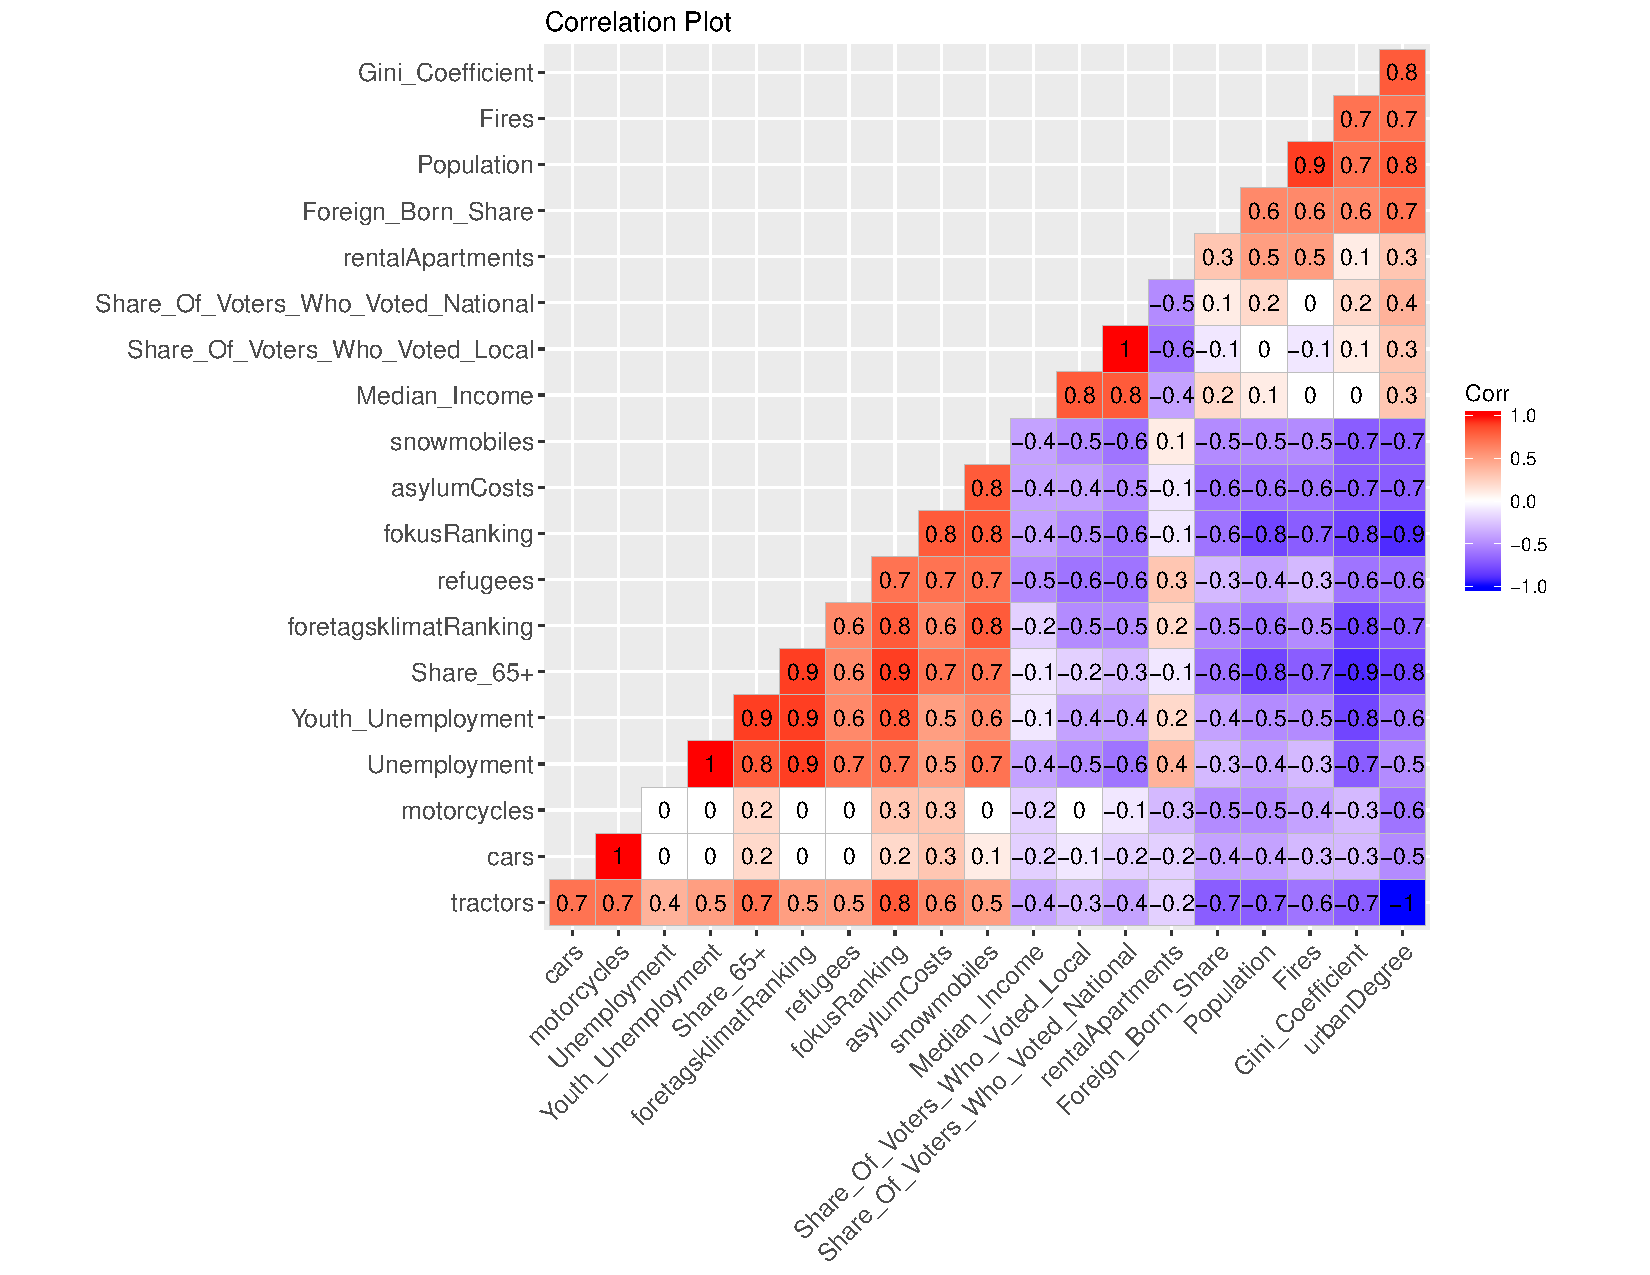
\includegraphics[width=1\linewidth]{../fig/corr_plot}
	\end{minipage} \hfill
	\begin{minipage}[c]{0.29\textwidth}
	\caption{Correlations between the 25 predictors can be also be quite high.  For example, the correlation between the population of automobiles and that of motorcycles is over 0.89.  Even less obviously related metrics like the Fokus rating and youth unemployment have a correlation of 0.44.}
	\end{minipage}
	\label{fig:firespermuni}
\end{figure}

The Bayesian priors we employ will perform regularizations to control for this, and aid us in selecting the most important of our larger number of predictors.  Additionally, they can allow us to incorporate prior knowledge about the values of the parameters and intercepts- potentially useful given the economic and demographic domain.

\subsection{Data Exploration}


\begin{figure}[H]
	\centering
	\begin{minipage}[c]{0.7\textwidth}
		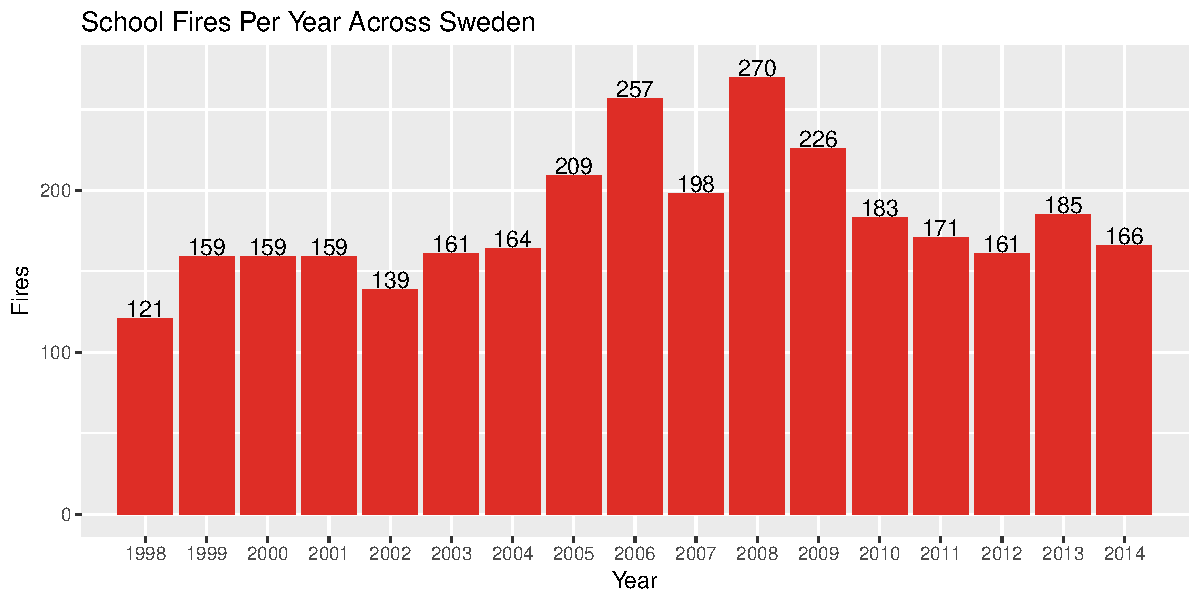
\includegraphics[width=1\linewidth]{../fig/FiresPerYear}
	\end{minipage} \hfill
	\begin{minipage}[l]{0.29\textwidth}
		\caption{Fires per year. We note that the years 2006 and 2008 were apparent outliers. Allowing our intercepts to vary will hopefully account for this effect and not bias our results.}
		\label{fig:firesperyear}
	\end{minipage}
	\begin{minipage}[c]{0.7\textwidth}
		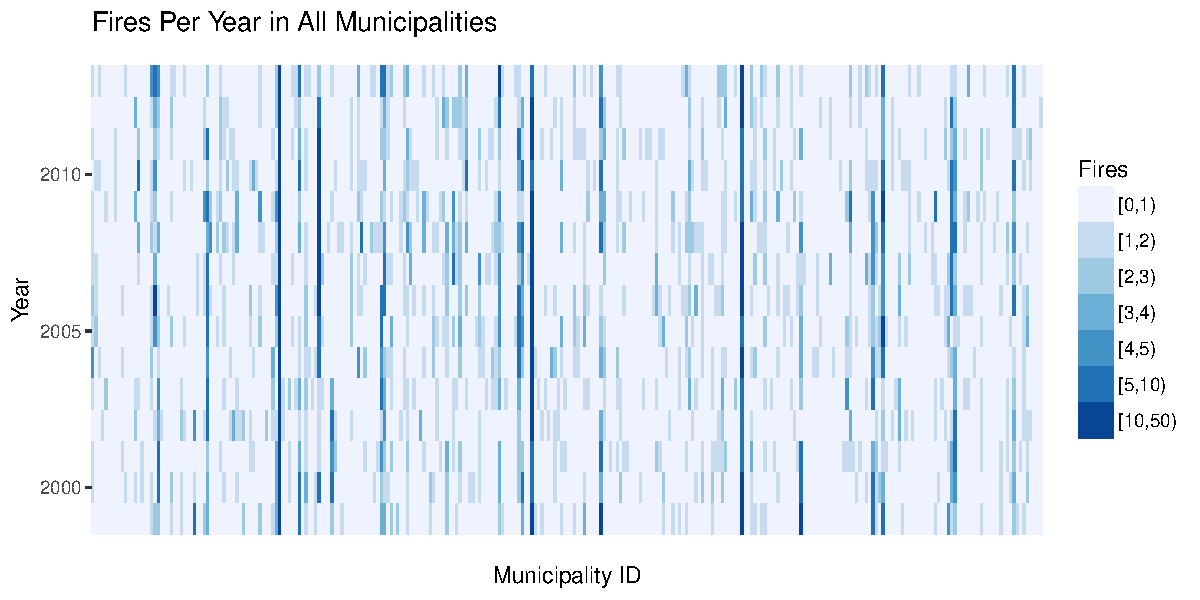
\includegraphics[width=1\linewidth]{../fig/FiresPerMuni_tile}
	\end{minipage} \hfill
	\begin{minipage}[l]{0.29\textwidth}
		\caption{Fires per municipality over time. Some municipalities, like those in the center, have a frequent number of fires per year, and others have almost none (lighter colors)}
		\label{fig:firespermunitile}
	\end{minipage}
	\begin{minipage}[c]{0.7\textwidth}
		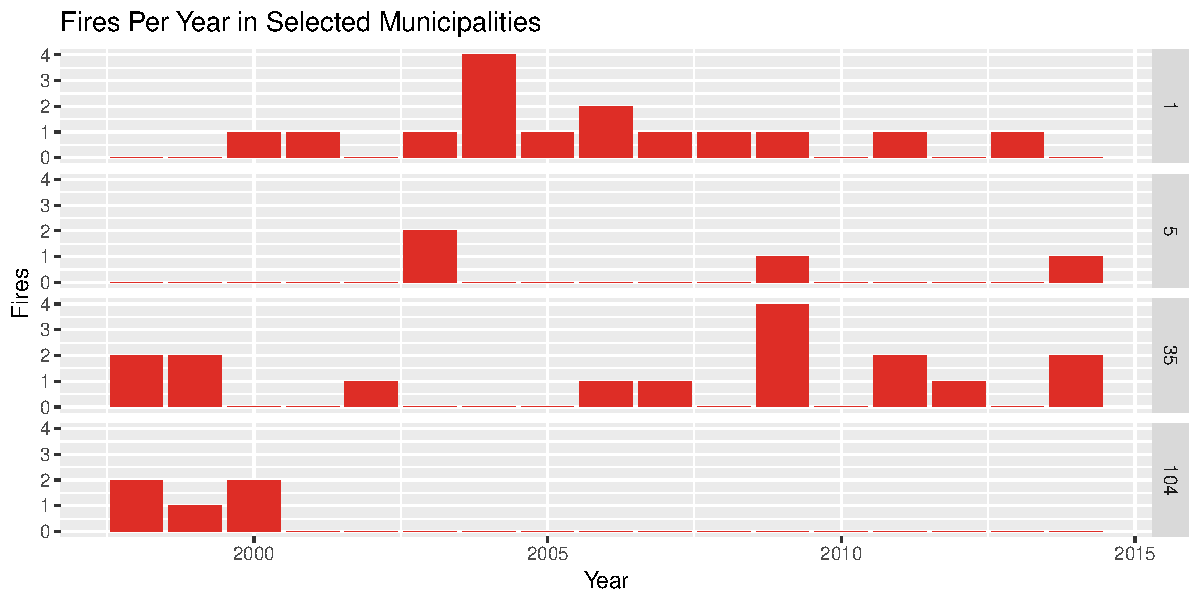
\includegraphics[width=1\linewidth]{../fig/FiresPerMuni}
	\end{minipage} \hfill
	\begin{minipage}[l]{0.29\textwidth}
		\caption{Fires over time for select municipalities. The variability in fires for each municipality is quite noticeable}
		\label{fig:firespermuni}
	\end{minipage}
\end{figure}


While fires over time show a relatively stable trend (see Figure \ref{fig:firesperyear}, \ref{fig:firespermunitile}, and \ref{fig:firespermuni}), among the municipalities, there is a great amount of variation. While nearly every municipality has at least one fire between 1998 and 2014, a smaller number of municipalities account for the majority of the fires. For example, in 2006, one municipality had 48 school fires. This will pose a challenge when modeling to account for the high amount of between- and within- municipality variance. The data is also very heavily biased for low numbers of fires per year. Over 97\% of the data has less than or equal to three fires, and so our model will need to work at both extremes - no fires and lots of fires. 

\subsection{Geographic Analysis}

Many of our predictors relate to measures of city scale and density, and anecdotally there does seem to be some connection between how rural or urban a municipality is and the incidence of school fires.  Accordingly, we began our analysis by making a heat map of school fires across Sweden. \\

\begin{figure}[H]
\centering
\begin{subfigure}{.5\textwidth}
	\centering
	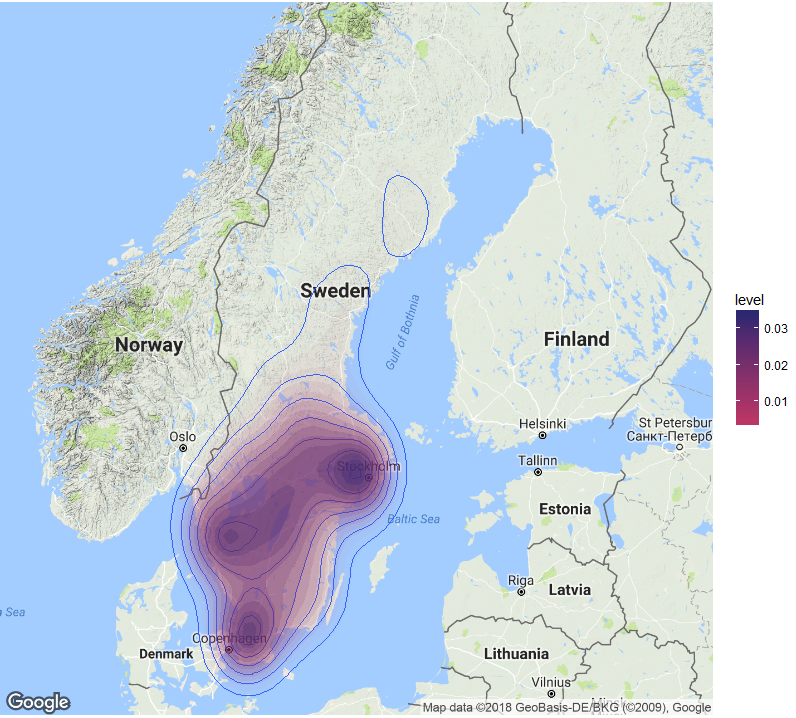
\includegraphics[width=0.9\textwidth]{../fig/HeatmapPoly.png}
	\caption{Heatmap of Sweden}
	\label{fig:sub1}
\end{subfigure}%
\begin{subfigure}{.5\textwidth}
\centering
	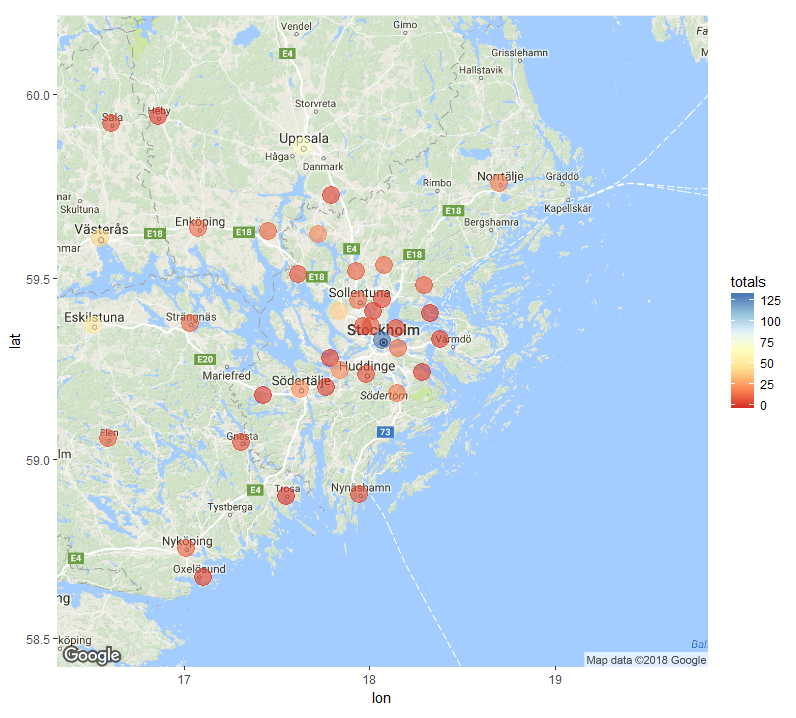
\includegraphics[width=0.9\textwidth]{../fig/HeatmapStockholm.png}
	\caption{Heatmap of Stockholm and Surrounding Areas}
	\label{fig:sub2}
\end{subfigure}
\label{fig:test}
\end{figure}

At first glance, it appears that school fires are more predominant around the more populated coastal areas in the south of the peninsula, particularly around the largest cities of Stockholm, Gothenburg, and Malm{\"o}. Examining the area around capital of Stockholm more closely, we find interestingly that the municipalities more strongly impacted by school fires appear to, paradoxically, be in the less populated suburbs.

\subsection{Preliminary Regression and Key Predictor Interpretations}

For a preliminary assessment of predictor-outcome relationships, we ran some initial Bayesian regressions within a specific slice of time, prior to the full model incorporating year-to-year differences. Due to the relative sparsity of the outcome, we selected aggregate school fires in the 2010-2014 period as an outcome.\footnote{This period was selected due to a) the relative richness of predictor data in this period and b) the fact that Sweden's overall economic conditions were fairly consistent across this period, without much volatility.} After comparing a handful of models for accuracy, run time, and interpretability, we settled on a fairly basic model specification below:
\begin{align*}
Fires_{muni} \sim Poisson(\lambda) \\
log(\hat{\lambda}) = \beta_0 + \sum\nolimits_{i=1}^V \beta_iv_i \\
\beta_1,...,\beta_V \sim N(0,1)
\end{align*}
Where subscript $muni$ refers to a given municipality, and $V$ is the total number of parameters.

Preliminary model plots are shown in Figure \ref{fig:sub1} and \ref{fig:sub2}. Our results and plots provide moderate evidence that suburban areas, with higher populations but not peak population densities see the highest occurrence of school fires. More tractors and snowmobiles, proxies for rurality, correlate with fewer school arsons. 

Higher levels of urbanicity correlate with more school arsons, but this tails off near higher levels of density. More directly, the box-plot in Figure \ref{fig:sub2} shows that municipalities classified specifically as towns show the highest incidence of arson in the 2010-2014 period.

Additionally, we have evidence that poor economic conditions or a lack of a vibrant economy has a positive relationship with school arson. Unemployment and youth unemployment are both correlated (albeit weakly) with school arson. We also see that median income and the Gini Coefficient (which, as an inequality measure, will often \textit{increase} for cities with growing wealth), are both significantly negatively correlated with school arson.

\begin{figure}[H]
	\centering
	\begin{subfigure}{.6\textwidth}
		\centering
		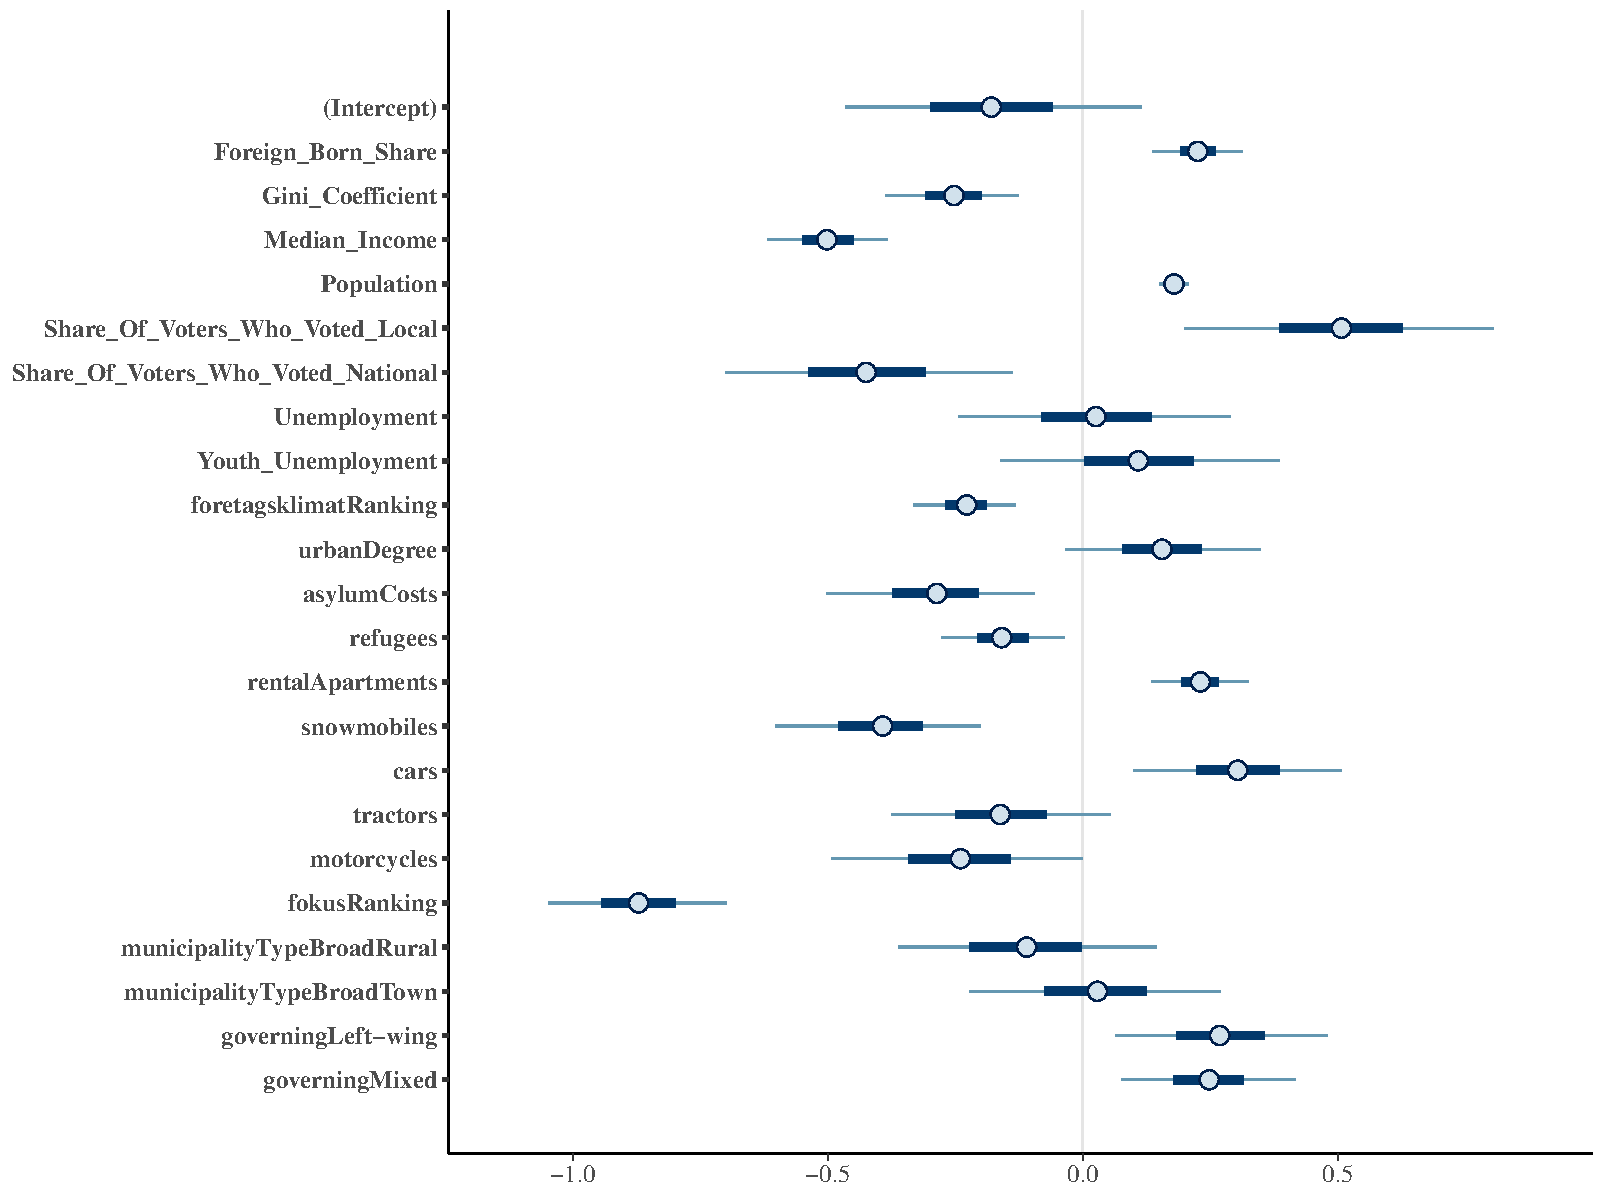
\includegraphics[width=0.9\textwidth]{../fig/parameterintervals}
		\caption{Uncertainty Intervals for Regression Parameters}
		\label{fig:sub1}
	\end{subfigure}%
	\begin{subfigure}{.4\textwidth}
	\centering
		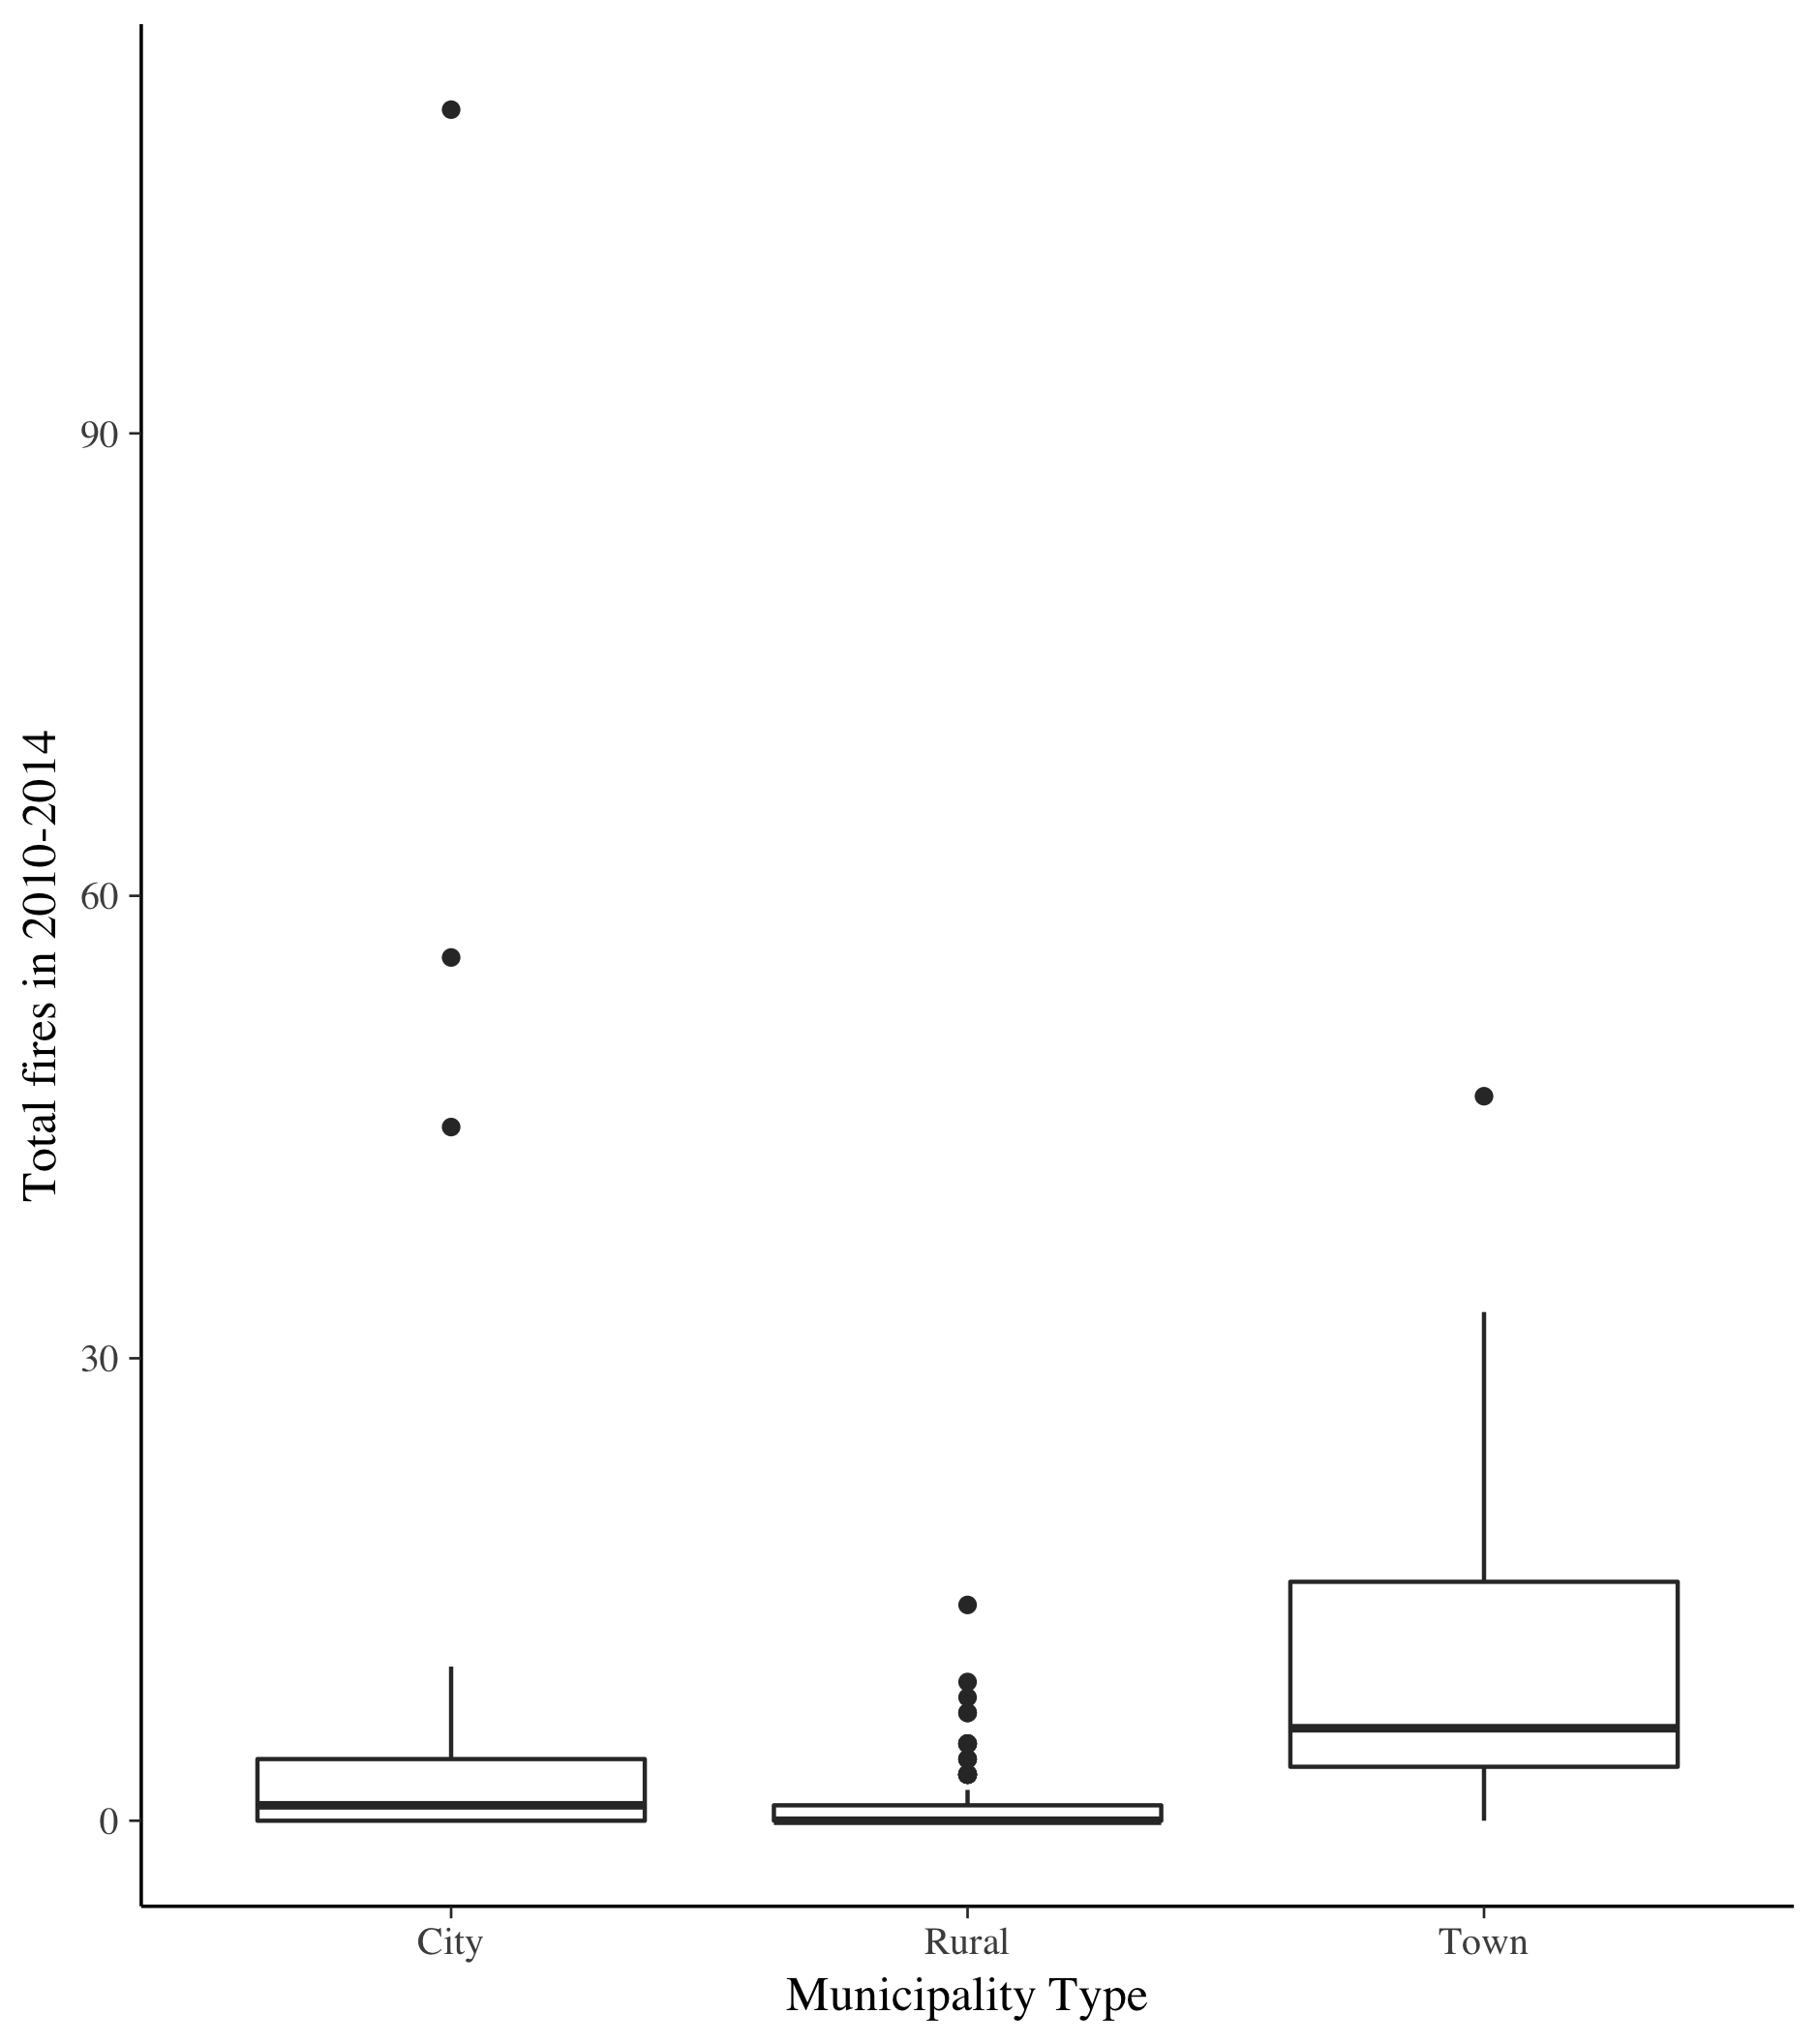
\includegraphics[width=0.9\textwidth]{../fig/muni_type_fires.png}
		\caption{Fires by municipality type}
		\label{fig:sub2}
	\end{subfigure}
	\label{fig:test}
	\caption{Preliminary Findings from Analysis of 2010-2014 Fires}
\end{figure}

Comparing this model structure with alternatives yielded little deviation in performance. The table in Table \ref{table:ELPDmodels} shows a quick comparison of two models in terms of their estimated expected log predictive density (ELPD), a measure of predictive accuracy. Estimating it enables comparison of model performance -- a higher estimated ELPD suggesting a higher out-of-sample predictive performance.
%
\begin{align*}
ELPD = \sum_{i=1}^nE_f\left[\log p_{post}(\tilde{y_i})\right] = \sum_{i=1}^n\int \log p_{post}(\tilde{y_i}) \, d\tilde{y}
\end{align*}
Comparing the 5-fold cross-validated model without random effects (summarized above) against a model with random effects (on different governing structures and municipality types) shows little meaningful difference in performance. The random effects model, additionally, has a higher run time. 

\begin{table}[H]
\centering
\begin{tabular}{rr}
  \toprule
  No.RE & With.RE \\ 
  \midrule
 -465.92 & -579.52 \\ 
   \bottomrule
\end{tabular}
\caption{Comparison of Models with and without Random Effects} 
\label{table:ELPDmodels}
\end{table}

\section{Bayesian Modeling Framework}

\subsection{Early Modeling Attempts}
\subsubsection{Improving the Fit}
We took a step-wise approach to avoid building too complicated a model that would potentially overfit the data.  We aimed to keep our model as simple as possible for reasons of both computation and interpretation, and consequently updated it over several iterations. 

We began with a fixed effects, fixed intercepts model which was easily implemented in Rstanarm. We then realized that the variability in municipalities required a different model - one with varying intercepts for the municipalities as so we moved to STAN to implement this model. The outlier years in 2006 and 2008 were problematic in that the observations in these years were not being captured in our posterior predictive distribution, and so we incorporated a third term (the year intercepts) to account for the fact that some years had more fires than others. 

Correlation in the predictors, and our ignorance as to what features should be implemented, allowed regularization priors to be implemented in the next model, which greatly reduced the bouncing betas that we were seeing in the predictors. However, divergence issues and weakly informative data forced us to re-parameterize our model to move the correlation from the parameters (the estimation of the slopes) into the hyperparameters - this is talked about more in the next section. 

We decided, at last, to settle on a mixed-intercepts fixed effects model for both reasons of interpretation, computation, and it performed very well at recovering the original data in the model checking phase. We used regularization priors, and we will discuss this model in the sections to come. 

We also attempted to fit a zero-inflated Poisson mixture model to account for the fact that many of the municipalities had zero fires in a given year. After looking at the improvement in fit, and weighed against the very large increase in both computation time and implementation difficulty, however, we decided against using the more complicated mixture model, and instead prefer the mixed-intercepts model for ease of computation and interpretation\footnote{Please refer to our posterior predictive summaries in the model checking phase to see that the model is flexible enough to account for the zero-inflated data at the municipality level.}. 

\subsubsection{Divergence, Hierarchical Funnels, and ``Matt's Trick''}
As a consequence of hierarchical modeling, and the design of the NUTS algorithm (No U-Turn Sampler: reliant on the gradient and the Hessian of posterior space), hierarchical models are prone to divergence issues when the data is not strongly informative or when the sample size is small. Such issues are commonly known as \textit{Neal's Funnel}. As is the case with most economic data, the amount of noise present in our data from correlated predictors and observations, inherent census sampling errors, and our economic predictors being lagging indicators, we had divergence issues plague our initial models - especially those that used centered parameterizations. 

As a consequence of the geometry of the posterior space, we had to implement ``Matt's Trick'' (a non-centered parameterization method) to tame the posterior and move the model correlations in the parameters over to the hyper-parameters. We used the non-centered parametrization of the double exponential distribution to regularize most variables, along with the fact that it is a location-scale family, to rework our parameterization as suggested in \cite{stanmanual} and \cite{benacourt}. This solved all of our divergence issues, and ultimately allowed the sampler to work much more efficiently.

\subsection{Description of the model}

\newcommand{\munis}{\ensuremath{muni}\xspace}
\newcommand{\years}{\ensuremath{year}\xspace}
\newcommand{\vars}[1]{\ensuremath{variable_{#1}}\xspace}
\newcommand{\indic}[2]{\ensuremath{\mathbb{I}\left[#1 = #2\right]}\xspace}

Our final model was a mixed-intercepts, fixed slopes model with shrinkage priors\footnote{See \cite{stantutorial} for a discussion on mixed effects models and Page 527-528 of \cite{stanmanual} for a non-centered parameterizations for a Double Exponential distribution to avoid divergence issues. }. 
%
\begin{align*}
	\beta_0 &\sim N(\mu_{(Intercept)},\sigma_{(Intercept)}) \quad \text{[Intercept Prior]}\\
	\beta_{(\vars{i})} &\sim Laplace(0, \sigma_{\vars{i}}) \quad \text{[Regularization Prior]}\\
	\beta_{(\years)} &\sim Laplace(0, \sigma_{\years}) \quad \text{[Regularization  Prior]}\\
	\beta_{(\munis)} &\sim Laplace(0, \sigma_{\munis}) \quad \text{[Regularization Prior]}\\
	\lambda_{\munis, \years} &= \beta_0 + \beta_{(\munis)} + \beta_{(\years)} + \sum\nolimits_{i = 1}^{V} \beta_{(\vars{i})} \vars{(i, \years)}\\
	Fires_{\munis, \years} &\sim Pois\left(\exp\left[\lambda_{\munis, \years}\right]\right)
\end{align*}

The final model contains several priors in order to account for the variables in the data.  Now adjusting for different mean fires across 17 year and over 250 municipality intercepts, alongside the 25 socioeconomic predictors, our model estimates over 4000 means.  While our preliminary model treated time as 'flat', ignoring that dimension, this model takes temporal changes into account. It also aims to manage the natural propensity of some municipalities to have a disproportionate number of fires outside of what we predict. The mixed-intercepts account for these two sources of bias. Additionally, by using regularizing priors, we can limit the dramatic, sensitive changes in predictor coefficients that would occur in a standard regression framework, hopefully providing for more stable and accurate predictions. The greatest challenge of this model is going to be picking up the outliers in the data - over 97\% of the data has less than or equal to three fires a year and so we need to have a model sensitive enough to work in the tails as well.

\section{Modeling Results}
\subsection{Convergence and Model Checking}

After running the model, we ran ShinyStan to perform most of the model checking steps. We had effective sample sizes all greater than 40\% of the total sample size, and we averaged about 90\% efficiency on an \textit{effective samples / total samples} basis. There were no messages for divergence of the chains (see Matt's Trick above), and the tree-depth was not exceeded on any of the runs. R-hat was never more than a rounding error above 1.00. The energy for each of the chains was consistent as well, indicating that each chain was exploring a similar geometry. We have elected to omit figures for the graphical model checking for the purposes of brevity, but they are available on request and we saved our model object if you would like to investigate further. 

We, now, need to check that the posterior predictions cover our response variable in most cases. If the posterior predictive distribution fails to capture our data, our model may not be rich enough to express the nuances in the data. 

\begin{figure}[H]
	\centering
	\begin{minipage}[c]{0.6\textwidth}
	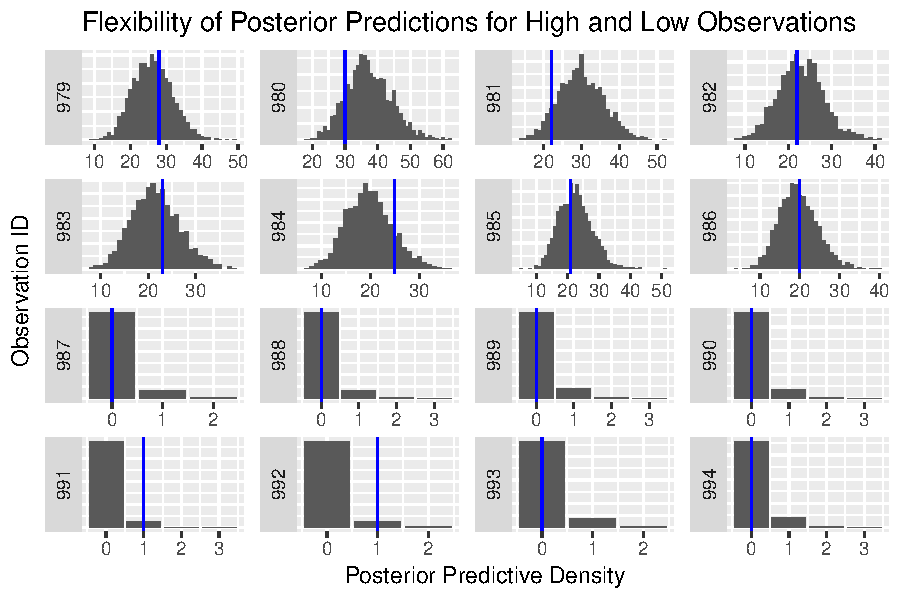
\includegraphics[width=\textwidth]{../fig/post_pred_samples}
	\end{minipage} \hfill
	\begin{minipage}[c]{0.39\textwidth}
	\caption{Histogram of fire counts. The first eight observations (on top) are from a municipality with a lot of fires, and the bottom eight observations are from a municipality with a small amount of fires. }
	\label{fig:postpredsamples}
	\end{minipage}
\end{figure}

Looking at two different municipalities, in Figure \ref{fig:postpredsamples}, one with a high number of fires (top eight), and one with a low number of fires (lower eight), we can see that the posterior predictive distribution (histogram) covers the true number of fires (verticle blue line) in every case.

\begin{figure}[H]
	\centering	\begin{minipage}[c]{0.6\textwidth}
		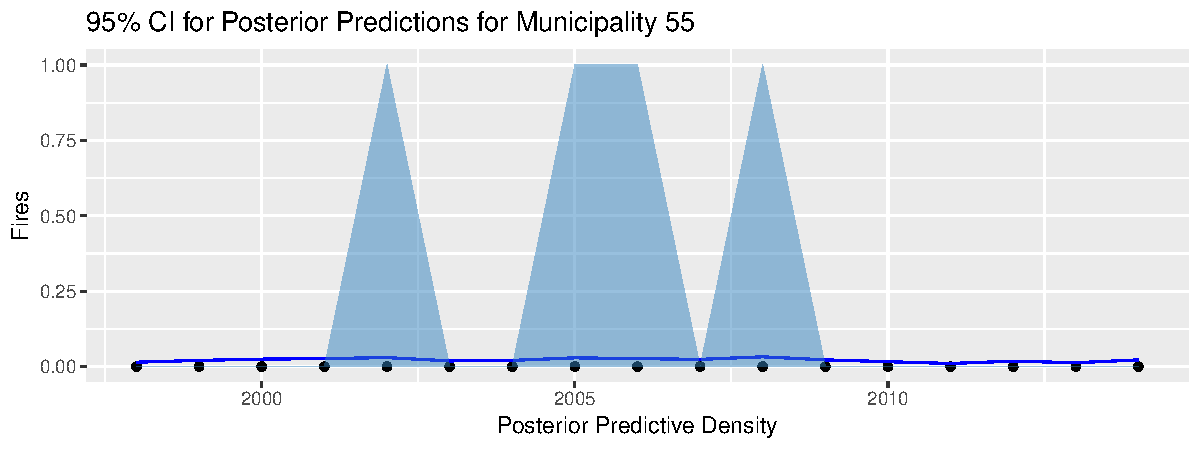
\includegraphics[width=\textwidth]{../fig/post_pred_samples_ribbon_low}
	\end{minipage} \hfill
	\begin{minipage}[c]{0.39\textwidth}
		\caption{Credible interval, municipality with few fires}
		\label{fig:lowfires_ribbon}
	\end{minipage}
	\centering	\begin{minipage}[c]{0.6\textwidth}
	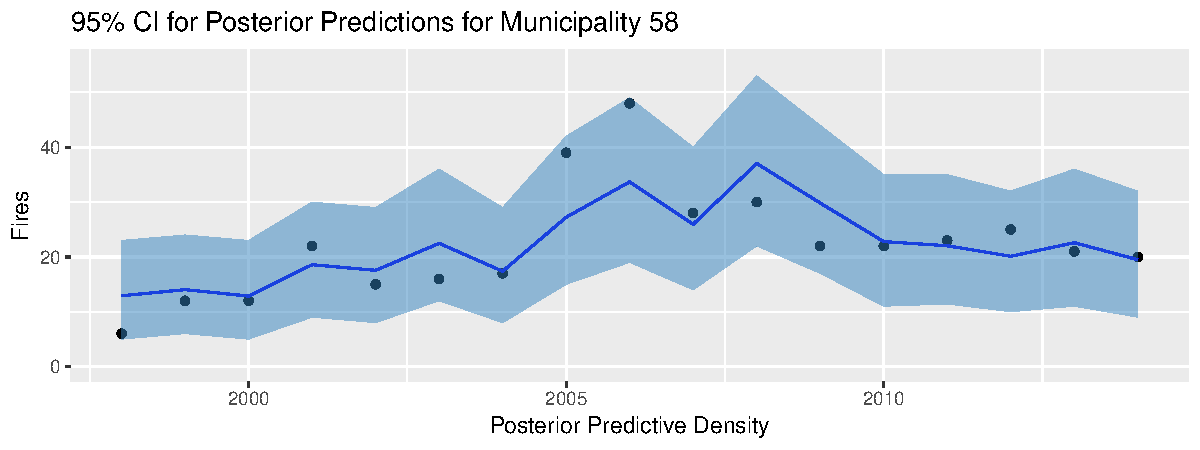
\includegraphics[width=\textwidth]{../fig/post_pred_samples_ribbon_high}
\end{minipage} \hfill
\begin{minipage}[c]{0.39\textwidth}
	\caption{Credible interval, municipality with many fires}
		\label{fig:highfires_ribbon}
\end{minipage}
\end{figure}

	Looking at Figure \ref{fig:lowfires_ribbon} and \ref{fig:highfires_ribbon}, for municipalities with a small amount of fires, the credible interval hovers between zero and one fire- this covers 100\% of the points in the first municipality (Figure \ref{fig:lowfires_ribbon}).  For municipalities with a large amount of fires, we can see that the credible interval also does a good job at capturing the number of fires. The width of the confidence intervals is largely a function of the over-dispersion that we have in our Poisson estimates as a function of the noise in our predictor variables and thus noise in our computation of $\lambda$.

\subsection{Graphical Analysis}
\begin{figure}[H]
	\centering
	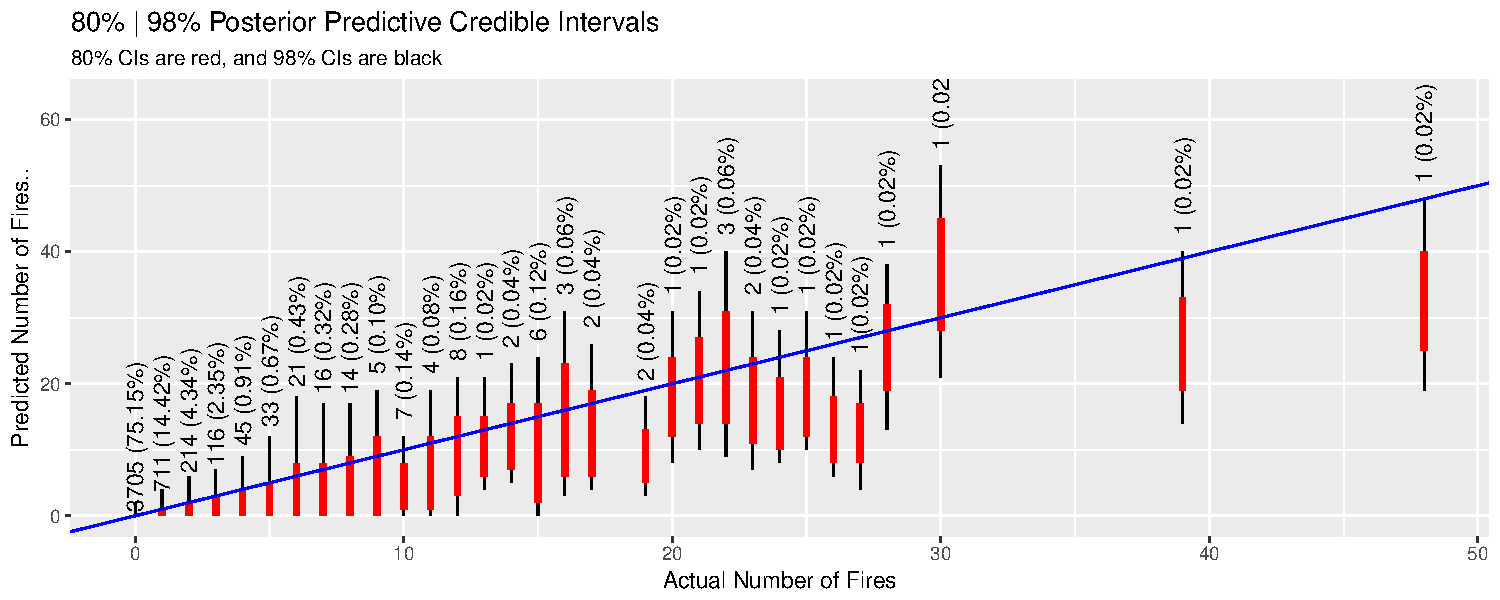
\includegraphics[width=1\linewidth]{../fig/CI_post_pred_intervals}
	\caption{Credible intervals, posterior predictive distribution.  The first number is the number of observations with that fire count, and the second is this number as a percentage of the total observations. Despite the incredibly rare occurrence of over 20 fires per year, our posterior intervals, in almost every case, manage to cover the true number of fires (blue line). This is impressive  considering just how bias the data is (97\% of our data points have less than or equal to three fires in a given year.)}
\label{fig:cipostpredintervals}
\end{figure}

We can see that most of the 98\% CI's contain the actual number of fires - indicating that the model was able to capture the nuances of the data, except for a handful of cases that were outliers (such as the two observations with 19 fires). When implementing the zero-inflated model, we noticed that the posterior intervals were slightly better at capturing the true observations of number of fires, but the computational concerns, and the fact that every CI now overweighted zero, meant that the CI's had a larger standard error because of the way that the CI was constructed. In future analysis, we would like to construct bi-interval CI's to account for the bimodal nature of a zero-inflated Poisson to see if this helps better the prediction.


\begin{figure}[H]
	\centering	\begin{minipage}[c]{0.6\textwidth}
		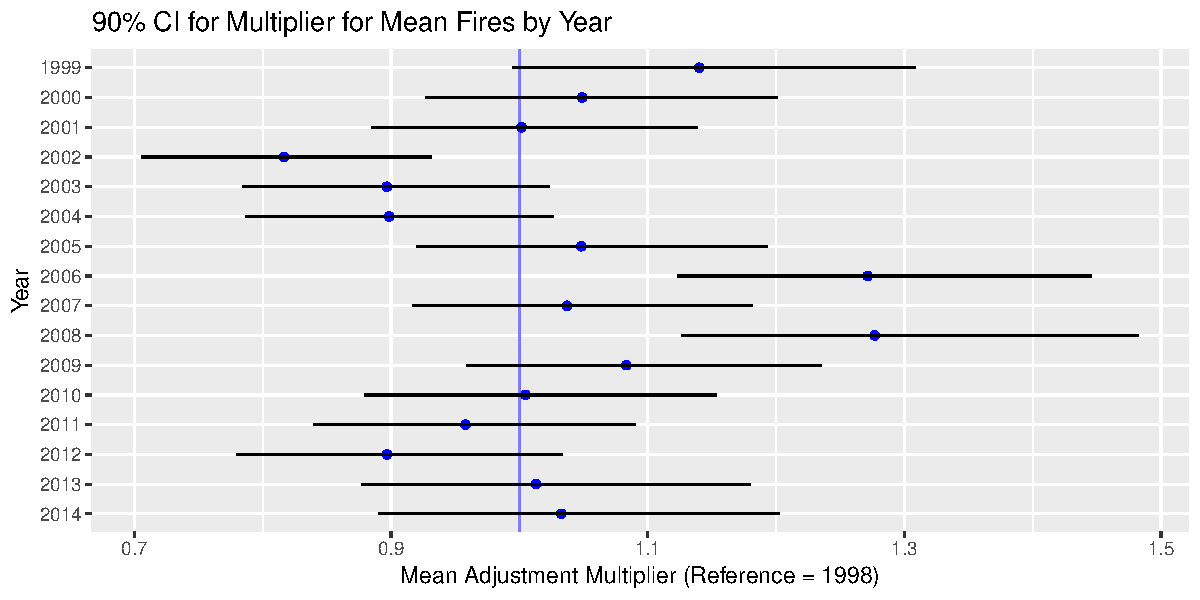
\includegraphics[width=\textwidth]{../fig/year_multiplier}
	\end{minipage} \hfill
	\begin{minipage}[c]{0.39\textwidth}
		\caption{Comparing Confidence Intervals for Mean Fires by Year, with reference year 1998}
	\label{fig:yearmultiplier}
	\end{minipage}
\end{figure}

When examining the year multiplier with reference year 1998, we see that very few years appear to be significantly different from the reference in terms of effect size.  In 2002, we bias the fires down 0.70x-0.90x relative to the 1998, and we correct them upwards in 2006 and 2008, both which were years with a relatively large number of fires. This would confirm some of our earlier intuition that the number of fires does not swing as dramatically from year to year as it does from municipality to municipality.

\begin{figure}[H]
	\centering
	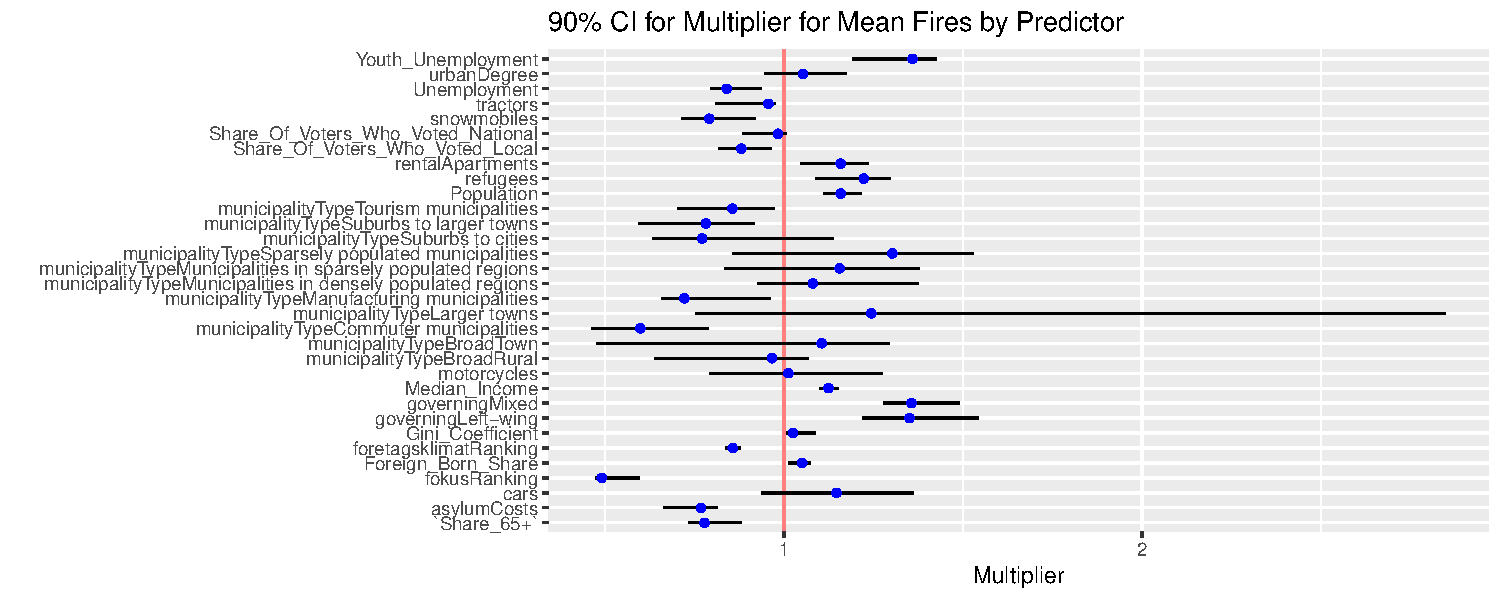
\includegraphics[width=1\linewidth]{../fig/beta_multiplier}
	\caption{Mean multiplicative factor for each of the predictors}
	\label{fig:betamultiplier}
\end{figure}

In the parameter intervals shown in Figure \ref{fig:betamultiplier}, now considering the full year-by-year analysis, we see some similarities (and some differences) from our preliminary model results. By controlling for the multiple observations on a given municipality, and controlling for the bias for fires to occur more or less frequently as a function of the year, we notice that the betas on the predictors have changed as a result. Importantly, youth unemployment now emerges as a major positive predictor, while general unemployment actually becomes a negative predictor. We also no longer see as clear a pattern in which suburban-level town types predict fire incidence, although municipalities classified as larger towns still show a boost in arson incidence. Note the significant uncertainty inherent in many of the municipality classification parameter estimates, which suggest that specific demographic and economic factors are the most relevant predictors of arson.


\section{Conclusion}
Sweden's school fires are a problem both unusual and unfortunate.  Like many cultural phenomena, they resist easy quantification, prediction, and understanding.  However, through Bayesian regression and hierarchical modeling, we have been able to isolate some correlates of schoolyard arson that make intuitive sense.  In both our preliminary and final models, measures of low economic conditions showed significance.  In particular, after expanding our model to include a time component (near-essential for economic data), youth unemployment specifically stood out.  Collectively, this suggests that limited opportunities for young people are associated with more frequent man-made fires in schools.

Additionally, increasing urbanicity and wealth (as measured by improved business rankings, median income, inequality, and increasing inflows of foreign-born residents) were also a notable beta.  This appeared especially true in areas of median population.  Together with the economic predictors, this suggests that Swedish school fires may be more comprehensible than we first suspected.  In the United States, as well as in many other countries, semi-urban environments with lower levels of economic activity are anecdotally associated with general, potentially short-lived, increases in low-level criminal behavior (e.g. vandalism, graffiti, etc).  It would appear that, in Sweden, this international practice extends to criminal arson in schools.

In addition to our conclusions regarding the problem in question, some learnings were also made regarding the model itself.  Very quickly, we found that the general rarity of school arson introduces estimate uncertainty.  The usual regression assumptions of uncorrelated errors were disrupted by year-to-year serial correlation and the multicollinearity of otherwise very useful economic data. Hierarchical modeling and regularization priors proved valuable tools in adjusting for this.

Lastly, the data leaves plenty of room for follow up.  We only scratched the surface of a deep well of predictors offered by the Swedish government, totaling over 2600 variables and offering many options to the interested analyst.  While this significant dimensionality poses considerable feature selection challenges, data mining approaches, along with model selection methods like the use of Bayes information criterion, could be useful in addressing these. 


\section{References}

\begingroup
\renewcommand{\section}[2]{}

\begin{thebibliography}{depth}
\bibitem{mice_ref}
	Azur, Melissa, Elizabeth A. Stuart, Constantine Frangakis, and Philip J. Leaf. "Multiple Imputation by Chained Equations: What is it and how does it work?" \textit{Int J Methods Psychiatr Res.} Mar. 2011.
\bibitem{benacourt}
	Betancourt, M. J.; Girolami, Mark. ``Hamiltonian Monte Carlo for Hierarchical Models''. December 2013.
\bibitem{data_source}
	Data available here: \url{https://www.kaggle.com/mikaelhuss/swedish-school-fires}
\bibitem{BDA_Gelman}
	Gelman, Andrew, John Carlin, Hal Stern, David Dunson, Aki Vehtari, and Donald Rubin. \textit{Bayesian Data Analysis: Third Edition}. CRC Press. 2014.
\bibitem{Swedish Fire Report}
	Johannson, Nils, Patrick van Hees, Margaret Simonson McNamee, Michael Str{\"o}mgren and Robert Jansson. "Fa{\c c}ade fires in Swedish school buildings." \textit{EDP Sciences}. 2013.
\bibitem{stanmanual}
 	Stan Modeling Language User's Guide and Reference Manual, Version 2.17.0. \url{https://github.com/stan-dev/stan/releases/download/v2.17.0/stan-reference-2.17.0.pdf} 

\bibitem{stantutorial}
	Vasishth, Shravan. ``Bayesian Linear Mixed Models using Stan: A tutorial for psychologists, linguists, and cognitive scientists''. \url{http://www.ling.uni-potsdam.de/~vasishth/statistics/BayesLMMs.html}. Stan Tutorials.
    
    
\end{thebibliography}

\endgroup

\newpage
\section{Code Appendix}

\subsection{Stan Model}
The following code is the script file for Stan. This is the sixth implemented model.
\lstinputlisting[language={}]{../code/swed_fires_model_six_new_data_doubleexp.stan}
\subsection{Stan Call Script and Visualizations}
The following code is responsible for running the stan model and producing the visualizations that are used in model checking, posterior predictions, and inference analysis. 
\lstinputlisting[language=R]{../code/Stan_call_script_new_data_lasso_model.R}

\subsection{Preliminary Model}
This is the code that runs the preliminary analysis for our models
\lstinputlisting{../code/PrelimModel.R}

\subsection{Code for Translating the KPI to English}
We had to translate the KPIs from Swedish to English. This code is responsible for this translation using the Google Translate API.
\lstinputlisting{../code/Translations.R}

\subsection{Refactoring Code}
This takes the Translated data and makes it into the panel data.
\lstinputlisting{../code/ExtractYearByYearVars.R}


\end{document}